\documentclass[graybox]{svmult}

\usepackage{booktabs}
\usepackage{cite}
\usepackage[bottom]{footmisc}
\usepackage[utf8]{inputenc}
\usepackage{graphicx}
% epstopdf needs to be included after graphicx.
\usepackage{epstopdf}
\usepackage{listings}
\usepackage{makeidx}
\usepackage{multicol}
\usepackage{newtxtext}
\usepackage{newtxmath}
\usepackage{url}
\RequirePackage[l2tabu, orthodox]{nag}

% Allow PDF 1.7 documents to be included with \includegraphics
\pdfminorversion=7

\graphicspath{{./img/}}

% listing
\lstset{%
  language={C},
  basicstyle={\small\ttfamily},%
  identifierstyle={\small\ttfamily},%
  commentstyle={\small\itshape},%
  keywordstyle={\small\bfseries},%
  ndkeywordstyle={\small\ttfamily},%
  stringstyle={\small\ttfamily},%
  frame={tb},%
  breaklines=true,%
  columns=[l]{fullflexible},%
  numbers=left,%
  numberstyle={\scriptsize},%
  stepnumber=1,%
  numbersep=1em,%
  lineskip=-0.5ex,%
  mathescape,%
  xleftmargin=2em,%
  framexleftmargin=1.5em,%
}

\makeindex

\begin{document}

\title*{An MPI Framework for HPC Clusters Deployed with Software-Defined
Networking}
% Use \titlerunning{Short Title} for an abbreviated version of
% your contribution title if the original one is too long
\author{Keichi Takahashi, Susumu Date, Yasuhiro Watashiba, Yoshiyuki Kido,
Shinji Shimojo}
% Use \authorrunning{Short Title} for an abbreviated version of
% your contribution title if the original one is too long
\institute{Keichi Takahashi \at Nara Institute of Science and Technology,
8916-5 Takayama, Ikoma, Nara, Japan\\ \email{keichi@is.naist.jp}
\and Susumu Date, Yasuhiro Watashiba, Yoshiyuki Kido, Shinji Shimojo \at
Cybermedia Center, Osaka University, 5-1 Mihogaoka, Ibaraki, Osaka, Japan\\
\email{{date, watashiba-y, kido, shimojo}@cmc.osaka-u.ac.jp}}
\maketitle

\abstract*{Each chapter should be preceded by an abstract (no more than 200
words) that summarizes the content. The abstract will appear \textit{online}
at \url{www.SpringerLink.com} and be available with unrestricted access. This
allows unregistered users to read the abstract as a teaser for the complete
chapter. Please use the 'starred' version of the \texttt{abstract} command for
typesetting the text of the online abstracts (cf. source file of this chapter
template \texttt{abstract}) and include them with the source files of your
manuscript. Use the plain \texttt{abstract} command if the abstract is also to
appear in the printed version of the book.}

\abstract{Each chapter should be preceded by an abstract (no more than 200
words) that summarizes the content. The abstract will appear \textit{online}
at \url{www.SpringerLink.com} and be available with unrestricted access. This
allows unregistered users to read the abstract as a teaser for the complete
chapter.\newline\indent Please use the 'starred' version of the
\texttt{abstract} command for typesetting the text of the online abstracts
(cf. source file of this chapter template \texttt{abstract}) and include them
with the source files of your manuscript. Use the plain \texttt{abstract}
command if the abstract is also to appear in the printed version of the book.}

\section{Introduction}

The demand for computing performance of high-performance computing (HPC)
systems has been every-growing. In fact, exascale HPC systems are now on the
horizon. To meet the sustained growth of HPC systems, the high-performance
network that interconnects the computing nodes composing a cluster, or
\textit{interconnect}, needs to be enhanced to achieve larger scale, higher
bandwidth and lower latency. As a result, the interconnect now accounts for a
significant portion of total financial cost and power consumption of an HPC
system~\cite{Michelogiannakis2017}.

Until today, the established strategy to design a interconnect has been
\textit{over-provisioning}, where bandwidth and routes are over-provisioned to
accommodate any application with arbitrary communication pattern will not
experience degradation of communication performance. The reason for this
choice is two-fold: first, a production HPC system is usually shared by many
users, where each user runs different applications. Therefore, it is not
realistic to tailor an interconnect to a communication pattern of a single
application. Second, conventional networking hardware used in interconnects do
not allow administrators to change their configuration on-the-fly. Therefore,
the only choice is to over-provision the interconnect with abundant bandwidth
and routes. However, an over-subscribed design is becoming increasingly
challenging to implement due to its rapidly rising financial cost and power
consumption. We believe that dynamically controlling the traffic in the
interconnect based on the communication pattern of an application could
overcome this problem.

However, with the recent emergence of networking technologies that introduces
programmability into networks, the assumption that interconnects are static
and cannot be reconfigured does not hold anymore. A prominent example of such
networking technology is Software-Defined Networking (SDN), which is a novel
networking architecture that allows administrators to dynamically and flexibly
control the network like a software.

Based on this idea, we have been developing on \textit{SDN-enhanced MPI}, a
framework that integrates Software-Defined Networking (SDN) into Message
Passing Interface (MPI). The goal of this framework is to dynamically control
the traffic in the interconnect based on the MPI communication pattern of
applications by utilizing the network programmability provided by SDN\@. To
this end, we have demonstrated that individual MPI collectives are accelerated
by utilizing SDN~\cite{Dashdavaa2014,Takahashi2014}. In addition, we have
designed and implemented a mechanism to synchronize the progress of an
application and the reconfiguration of the
interconnect~\cite{Takahashi2015,Takahashi2018}. Furthermore, we have
developed a toolset consisting of (1) a profiler to extract communication
pattern from applications and (2) an interconnect simulator predict the
traffic flow generated in an interconnect~\cite{Takahashi2017}.

Although our work so far has demonstrated that individual MPI applications can
be accelerated through the application of SDN, a key issue has remained
towards the deployment of our framework on production clusters: our current
SDN-enhanced MPI framework does not allow the concurrent execution of multiple
applications on a cluster. As mentioned earlier, clusters are usually shared
among many users. Therefore, it is crucial that multiple jobs are able to be
executed at the same time on a cluster.

In this paper, we aim to solve this limitation by integrating our framework
into the job scheduler of a cluster.

The rest of this paper is organized as follows. Section~\ref{kt:sec:ii}
describes the key technologies behind the proposal and challenges to be tackled.
Section~\ref{kt:sec:iii} proposes the architecture of the proposed framework.
Section~\ref{kt:sec:iv} shows the preliminary evaluation result of the
proposed framework. Section~\ref{kt:sec:v} concludes this paper and discusses
future work.

\section{Background}\label{kt:sec:ii}

\subsection{Software-Defined Networking (SDN)}

Software-Defined Networking (SDN)~\cite{Jamalian2015} is a novel networking
architecture that brings programmability into the network and allows users to
dynamically and flexibly control the network as if the network was a software.
In conventional networking architectures, the \textit{control plane}, which
makes the decision on how to handle packets, and the \textit {data plane},
which forwards packets, are tightly coupled together on each networking device
such as a switch. In SDN, the two planes are separated into different
hardware. Whereas data plane is implemented on each networking device, the
control plane is handled by a centralized software controller. Administrators
can achieve dynamic and flexible control over the network by developing a
controller that implements their desired control strategy.

The current de facto standard implementation of SDN is
OpenFlow~\cite{McKeown2008}. In an OpenFlow network, the data plane is handled
by OpenFlow switches, and the control plane is handled by an OpenFlow
controller. Switches and controllers communicate with one another through the
OpenFlow protocol. In this paper, we assume that the interconnect of the
cluster is deployed with OpenFlow switches.

\subsection{Job Scheduler}

A job scheduler is a system that manages the computing resources such as CPU
and memory in a cluster. The job scheduler accepts \textit{job} submissions
from users, which is a request to run an application on the cluster and a set
of resource to run the application. The job scheduler allocates computing
resource in the cluster and launch the application on the allocated computing
resources. If there are not enough available resource in the cluster, the job
will queued for later execution. Job schedulers used in production HPC systems
include Slurm~\cite{Yoo2003}, PBS
Professional\footnote{\url{https://www.pbspro.org/}},
Torque\footnote{\url{https://www.adaptivecomputing.com/products/torque/}} and
UNIVA Grid Engine\footnote{\url{http://www.univa.com/products/}}. In this
paper, Slurm is assumed as it is one of the most widely adopted open-source
job schedulers.

\begin{figure}
    \centering
    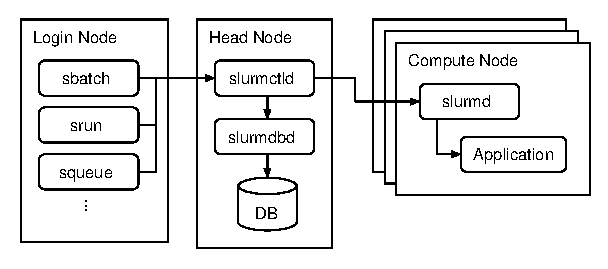
\includegraphics{slurm}
    \caption{Architecture of Slurm}%
    \label{kt:fig:slurm}
\end{figure}

Figure~\ref{kt:fig:slurm} shows the architecture of Slurm. Slurm employs a
\textit{master-worker} architecture like many other job schedulers. The
master, slurmctld, oversees the status of every compute node in the cluster.
It receives job submissions from users, allocates computing resources to a job
and launches the job by instructing to the workers. Optionally, slurmdbd is
used for logging and accounting purposes. Each compute node runs a worker,
slurmd, that monitors the status of the compute, communicates with slurmctld
and launches user applications when requested by slurmctld. Users interact
with slurmctld through utilities such as sbatch (submits a job), srun (submits
an interactive job) and squeue (list queued jobs).

\subsection{Challenges}


Since the job scheduler decided when to run which job,
. Furthermore,

\begin{itemize}
    \item Acquiring
    \item Node allocation and process mapping:
    \item Transparency from users:
\end{itemize}

\section{Proposal}\label{kt:sec:iii}

This section first briefly reviews the overall architecture of the proposed
framework. Subsequently, individual components of the framework are described
in detail.

\subsection{Overview}

Figure~\ref{kt:fig:architecture} shows the overall architecture of the
proposed SDN-enhanced MPI framework. The proposed framework mainly consists of
three components: (1) interconnect manager, (2) scheduler plugin, and (3)
OpenFlow controller. The interconnect manager is responsible for computing
optimized routes  for each job. The scheduler plugin is responsible
for sending information about a job when a job has started or finished. The
OpenFlow controller is responsible for communicating with the OpenFlow
switches and installing the routing generated by the interconnect manager.
We reuse a generic OpenFlow controller provided by the
Ryu\footnote{\url{https://osrg.github.io/ryu/}} OpenFlow framework that
provides a REST API to install, query, update and remove flows.

\begin{figure}
    \centering
    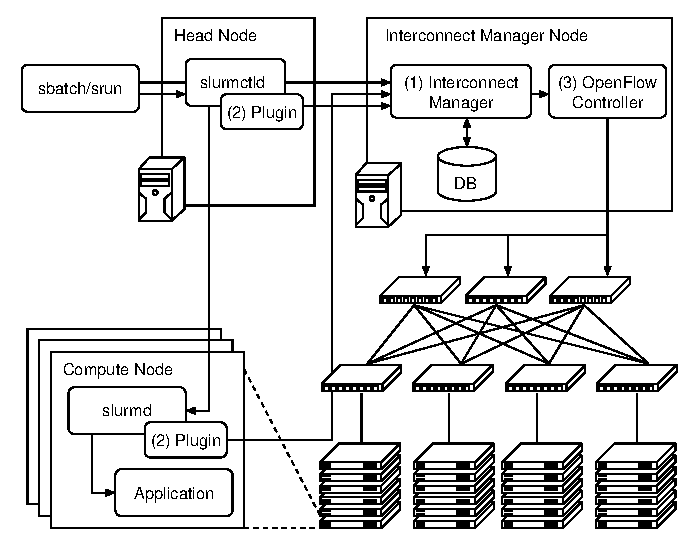
\includegraphics{architecture}
    \caption{Overall architecture}%
    \label{kt:fig:architecture}
\end{figure}

The scheduler plugin and the interconnect manager use RPCs to communicate with
one another. Specifically, gRPC\footnote{\url{https://grpc.io/}}, which is an
RPC framework built on top of HTTP/2, is used. The main reason behind this
choice is because gRPC can automatically generate server and client code from
an interface definition of remote procedures. Therefore, it saves much
implementation effort than implementing our own protocol on raw TCP/IP\@.

\subsection{Scheduler Plugin}

The scheduler plugin is responsible for sending information about a job when a
job has started or finished. As described earlier, the scheduler decides when
to run which job. Furthermore, the node allocation and process mapping are
unknown until the job starts. Therefore, a mechanism is needed to notify the
interconnect manager about these information.

For this reason, we utilize a builtin plugin mechanism of Slurm, which is
called Slurm Plug-in Architecture for Node and job Control (SPANK). SPANK
allows developers to easily customize the job startup and cleanup of Slurm.
SPANK plugins are not linked with Slurm itself and can be loaded during
runtime. In addition, SPANK allows developers to add new options to the job
script and job submission commands.

When a job is submitted by a user via sbatch or srun, our plugin sends the ID
and name of the job, uid of the submitter, number of processes and
communication pattern of the application to the interconnect manager. The user
needs to manually specify the communication pattern in the job script as shown
in Listing~\ref{kt:lst:script}.

\begin{lstlisting}[float,caption=An example of a job script,label=kt:lst:script]
#!/bin/bash
#
#SBATCH --job-name=cg-benchmark
#SBATCH --ntasks=128
#SBATCH --time=01:00:00
#
#SBATCH --comm-pattern=cg-c-128
\end{lstlisting}

When a job is being launched on each compute node by slurmd, our plugin sends
the ID and name of the job, node ID and MPI rank number to the interconnect
manager. These information is used by the interconnect manager to obtain the
node allocation and process mapping. After these information are sent over to
the interconnect manager, the plugin blocks until the routings are computed
and installed to the interconnect. Once the routings are ready, the plugin
returns control to Slurm and eventually, the user application is started.

When a job has finished, the same information is send over to the interconnect
manager. Similar to the launch, the plugin blocks until the routings are
uninstalled from the interconnect. After that, the rest of the cleanup is
resumed.

All of the above operations are performed transparently from the user
application. In other words, the user application does not need to be modified
nor a special program needs to be executed in the job.

\subsection{Interconnect Manager}

The interconnect manager is responsible for computing and installing optimal
routes for each job.

\begin{itemize}
    \item Receiving notifications from the scheduler plugin
    \item Maintaining the state of the cluster
    \item Computing optimal routing for each job
    \item Installing the computed routing to interconnect
\end{itemize}

SQLite\footnote{\url{https://www.sqlite.org/index.html}}

\section{Evaluation}\label{kt:sec:iv}

In this section, we conduct a preliminary evaluation to assess the
effectiveness of our proposed framework.

\subsection{Evaluation Environment}

The evaluation experiment was conducted on a small-scale cluster composed of
20 compute nodes connected through a two-tier fat-tree interconnect as
illustrated in Fig.~\ref{kt:fig:cluster}. Each compute node is equipped with
two quad-core Intel Xeon E5520 CPUs.

\begin{figure}
    \centering
    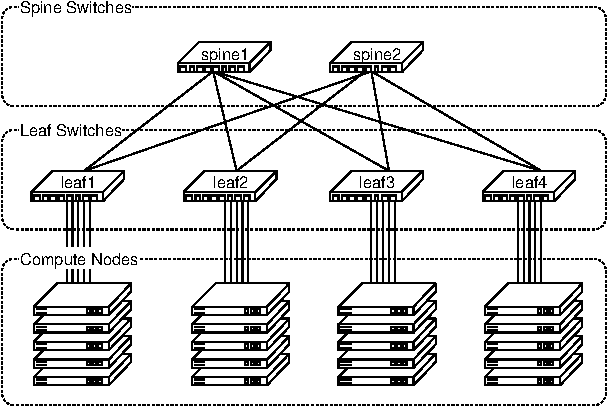
\includegraphics{evaluation_cluster}
    \caption{Cluster used for evaluation}%
    \label{kt:fig:cluster}
\end{figure}

\begin{table}
\caption{Kernels used in the evaluation}%
\label{kt:tbl:openflow-messages}
\begin{tabular}{ll}
\toprule
Name      & Description \\ \midrule
CG        & Solves a sparse linear system using the conjugate gradient method \\
LU        & Solves a dense linear system by using LU decomposition            \\
FT        &             \\
Stencil2D & A two-dimensional stencil solver           \\
Stencil3D & A three dimensional stencil solver            \\
Butterfly &             \\
SpMV      & A sparse-matrix vector kernel            \\ \bottomrule
\end{tabular}
\end{table}

\subsection{Evaluation Result}

\begin{figure}
    \centering
    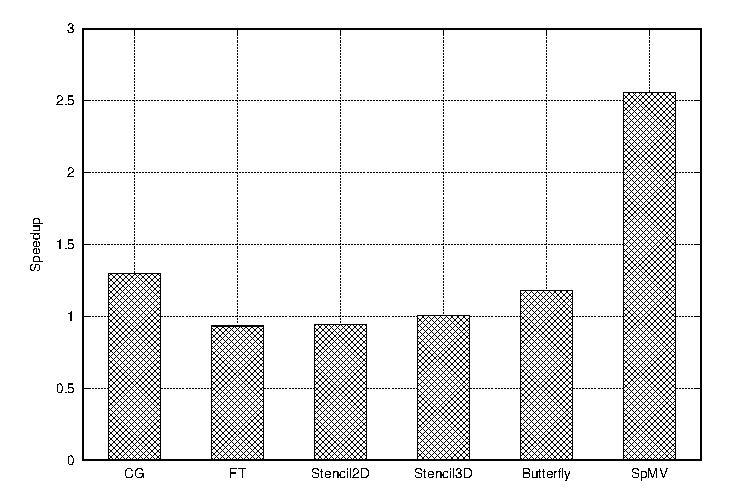
\includegraphics{benchmark_result}
    \caption{Benchmark results using miniapps}%
    \label{kt:fig:benchmark}
\end{figure}

\section{Conclusion}\label{kt:sec:v}

\begin{acknowledgement}
This work was supported by JSPS KAKENHI Grant Number 17K00168.
\end{acknowledgement}

\bibliographystyle{spmpsci}
\bibliography{references}

\end{document}
